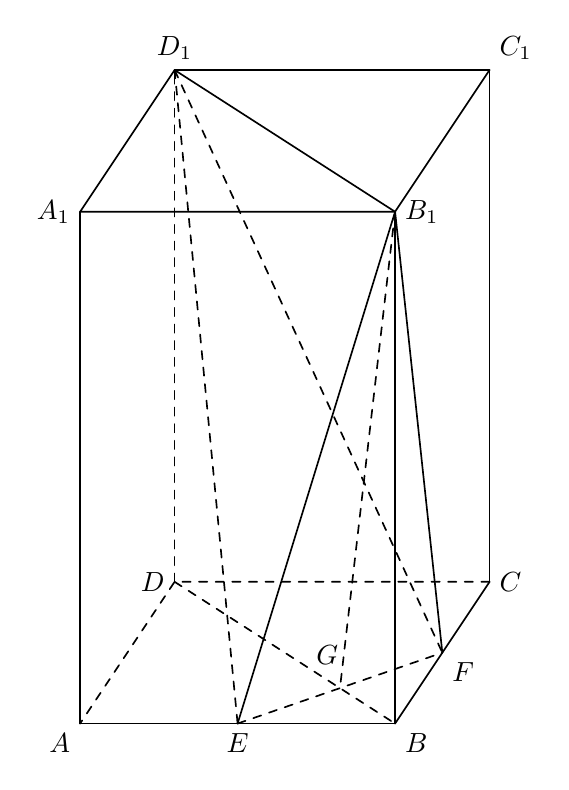
\begin{tikzpicture}[line width=0.6pt, line join=round, line cap=round]
  \coordinate (A) at (0,0);
  \coordinate (B) at (4,0);
  \coordinate (E) at (2,0);
  \coordinate (D) at (1.2,1.8);
  \coordinate (C) at (5.2,1.8);
  \coordinate (F) at (4.6,0.9);
  \coordinate (G) at (3.3000000000,0.4500000000);
  \coordinate (A1) at (0,6.5);
  \coordinate (B1) at (4,6.5);
  \coordinate (D1) at (1.2000000000,8.3000000000);
  \coordinate (C1) at (5.2000000000,8.3000000000);
  % bottom face
  \draw (A) -- (E) -- (B);
  \draw (B) -- (F) -- (C);
  \draw[dashed] (C) -- (D) -- (A);
  \draw[dashed] (D) -- (B);
  \draw[dashed] (E) -- (F);
  % verticals
  \draw (A) -- (A1);
  \draw (B) -- (B1);
  \draw (C) -- (C1);
  \draw[dashed] (D) -- (D1);
  % top face
  \draw (A1) -- (B1) -- (C1) -- (D1) -- cycle;
  % interior solid
  \draw (D1) -- (B1);
  \draw (E) -- (B1);
  \draw (B1) -- (F);
  % interior dashed
  \draw[dashed] (D1) -- (E);
  \draw[dashed] (D1) -- (F);
  \draw[dashed] (B1) -- (G);
  % labels
  \node[below left] at (A) {$A$};
  \node[below] at (E) {$E$};
  \node[below right] at (B) {$B$};
  \node[left] at (D) {$D$};
  \node[right] at (C) {$C$};
  \node[below right] at (F) {$F$};
  \node[above left,xshift=3pt,yshift=5pt] at (G) {$G$};
  \node[left] at (A1) {$A_{1}$};
  \node[right,xshift=0pt,yshift=0pt] at (B1) {$B_{1}$};
  \node[above] at (D1) {$D_{1}$};
  \node[above right] at (C1) {$C_{1}$};
\end{tikzpicture}
